\documentclass[12pt]{article}
\usepackage{graphicx}
\usepackage[utf8]{inputenc}
\usepackage[a4paper,left=2.5cm,right=2.5cm,top=2.5cm,bottom=2.5cm]{geometry}
\usepackage[frenchb]{babel}
\usepackage{setspace}
\onehalfspacing
\begin{document}

\begin{titlepage}
	\begin{minipage}{0.5\textwidth}
		\begin{flushleft}
			
\includegraphics[scale=0.1]{logo.png} \\
			\textbf{Département des sciences et génie}
		\end{flushleft}
	\end{minipage}
	\vspace{150px}
	\begin{center} \large
		\textbf{Connect Four : TP2} \\
		IFT-2003 \\
		Intelligence artificielle I \\
		\vspace{150px}
		\textbf{Destinataire} \\
		Laurence Capus
	\end{center}
	\vfill
	\rule{\linewidth}{.5pt}
	\newline
	\textbf{Catherine Asselin, 111 128 110} \\
	\textbf{Jérémie Lapointe, 111 008 937} \\
	\textbf{Patrick Voyer, 111 152 697} \\
	\textbf{Petru Lungu, 111 175 667} \\
\end{titlepage}

\newpage
\setcounter{page}{1}
\pagenumbering{arabic}

\section*{Introduction}
Le but de ce travail est de concevoir un jeu en utilisant des techniques d'intelligence artificielle, et ce, afin de mieux comprendre les différents concepts de l'intelligence artificielle. Notre équipe a choisi de concevoir le jeu de \textit{Puissance 4}, un jeu simple qui s'apparente au tic tac toe. Nous voulions créer un jeu qui se joue en duel avec l'ordinateur en utilisant un interface graphique de base. Nous avons réussi à créer une machine intelligence qui joue en fonction des mouvements du joueur, en plus de créer un jeu simple, mais amusant. Un guide d'utilisation ou ReadMe a été ajouté à la fin de ce document.

\section*{Présentation du jeu choisi}
Le jeu que nous avons choisi de concevoir est le célèbre jeu \textit{Connect Four} ou \textit{Puissance 4}. Ce jeu est composé d'un plateau à trous de 7 colonnes et de 6 rangées. Il est possible d'insérer des jetons par le haut du plateau dans chacune des colonnes. Le jeton inséré se retrouve alors au bas de la colonne. Un joueur a des jetons de couleur rouge (dans notre jeu, représenter par un 'x') et l'autre des jetons de couleur jaune (dans notre jeu, représenter par un 'o').\\

Le but du jeu est d'être le premier joueur à aligner 4 jetons de sa couleur sur n'importe quelle ligne ou diagonale du plateau. Chacun leur tour, les deux joueurs doivent mettre un jeton dans l'une des 7 colonnes du plateau, jusqu'à ce qu'il y est un vainqueur. Si toutes les rangées et colonnes sont pleines, et ce, sans qu'aucun des joueurs n'est aligné 4 jetons, la partie est déclarée nulle.

\section*{Modélisation du problème}

\subsection*{État initial}
L'état initial du jeux \textit{Puissance 4} sera représenté en utilisant des listes. Il y aura donc 7 listes qui permettront de représenter les différentes colonnes du jeu. Ces listes contiendront chacune 6 éléments pour représenter les emplacements ou peuvent être situé des jetons. Le début de la liste représentant le haut de la colonne (la première rangé à partir du haut) et la fin de la liste, le bas de la colonne (dernière rangée). De cette façon, nous obtenons un état initial qui a 7 colonnes et 6 lignes. Lorsque le jeu est initialisé, la valeur '-' est insérée dans chacun des 42 emplacements disponibles sur le jeu, et ce, afin d'indiquer que la case est vide. Par défaut, c'est le joueur qui commence la partie.

\subsection*{États finaux}
Les états finaux du jeu représentent toutes les combinaisons possibles pour qu’un joueur remporte la partie. Pour gagner une partie, un joueur doit avoir quatre jetons de sa couleur alignée sur une colonne, une rangée ou une diagonale. Dans notre cas, les jetons de couleur dont remplacé par les symboles 'x' et 'o'. Les états finaux doivent permettent de vérifier, à chaque tour joué si les jetons d’un joueur respectent une des 69 combinaisons possibles. Plus spécifiquement, notre jeu va vérifier après chaque mouvement effectué, si un joueur a gagné. Pour ce faire, une fonction prendra en paramètre le type de pion du joueur qui vient de poser une pièce (soit 'x', soit 'o') et la liste de liste qui représente le plateau de jeu. Celle-ci va alors parcourir toutes les combinaisons possible et voir si une des conditions gagnantes correspond à l'état actuel du plateau de jeu. Si une des conditions est respectée, le joueur qui viens de jouer est identifié comme gagnant et la partie se termine. Si aucune des combinaisons n’est identifiée, le joueur n’a pas gagné et c’est au second de joueur de jouer. 

Un des états finaux est que le plateau soit plein, soit qu'il y est soit un 'x' soit un 'o' sur toutes les cases, mais qu'aucun des deux joueurs n'Est gagné. Dans ce cas, la partie est déclarée nulle. Ainsi, après qu'un joueur est joué, notre jeu vérifier non seulement si le coup joué était un coup qui lui a permis de gagner la partie, mais il vérifie aussi si le plateau est plein. Si c'est le cas, la partie se termine, sinon c'est au joueur suivant de jouer.

\subsection*{Mouvements autorisés}
Le seul mouvement autorisé dans le jeu de \textit{Puissance 4} est l'insertion d'un jeton dans l'une des colonnes du jeu. Il existe seulement deux restrictions pour l'insertion d'un jeton. Tout d'abord, il faut que le joueur qui procède à l'insertion soit le joueur courant. La deuxième restriction est que la colonne dans laquelle le joueur veut insérer son jeton ne doit pas être pleine. C'est-à-dire qu'il ne faut pas qu'il y est déjà 6 jetons dans la colonne. Si c'est le cas, on indique au joueur que le mouvement n'est pas autorisé et il doit rejouer. \\

La première condition sera toujours respecté, car le jeu gère lui-même la rotation des joueurs, soit quel est le joueur qui doit jouer. Ainsi, le jeu fait en sorte que le joueur qui est choisi est toujours celui qui doit réellement jouer. Pour la deuxième condition, à chaque fois qu'un joueur choisira une colonne, il faudra vérifier s'il reste une case vide dans la liste représentant cette colonne. S'il y a une case de vide, le joueur pourra insérer son jeton dans cette colonne, sinon le joueur devra choisir une nouvelle colonne.

\subsection*{Technique de recherche}
La technique de recherche utilisée dans ce projet est la technique de min max. Le principe de la technique est que l'ordinateur est confronté à plusieurs choix. Il va alors noté tous les choix disponibles, et ce, considérant les gains pour le joueur qui joue et pour le joueur adverse. Le but sera alors de minimiser les gains pour l'autre joueur, considérant que le joueur adverse va joueur afin de maximiser ses gains. \\

Dans notre jeu, l'ordinateur a plusieurs options dépendant de ce qu'à jouer le joueur adverse. Si l'ordinateur voit que le joueur adverse peut gagner en jouant un jeton, l'ordinateur va ajouter un jeton à la colonne qui permet de bloquer le joueur adverse. En effet, si le joueur adverse a 3 jetons un par dessus les autres sur la colonne, l'ordinateur va détecté qu'il suffit au joueur d'ajouter un jeton sur cette colonne pour gagner. L'ordinateur va alors ajouter son jeton à lui sur cette colonne, pour réduire les chances de gagner de l'autre joueur. Si l'ordinateur détecte que le joueur adverse n'a pas de chance de gagner en ajoutant seulement un jeton, celui-ci va tenter de maximiser ses gains à lui en ajoutant un jeton pour le faire gagner. Si l'ordinateur ne détecte aucune chaine de 3 jetons pour le joueur adverse, il va regarder s'il peut gagner en ajoutant un jeton dans une des colonnes. Par exemple, si le joueur adverse a des jetons un peut partout, mais que l'ordinateur détecte qu'il a 3 jetons aligné dans la même rangé et qu'il peut ajouter un jeton dans une colonne pour avoir une rangée de 4 jetons alignés, l'ordinateur va jouer ce coup et lui permettre de gagner la partie. Si jamais l'ordinateur ne peut pas bloquer un coup gagnant de l'adversaire, ni gagner la partie en ajoutant un seul jeton, l'ordinateur va tenter de ralentir le joueur adverse. En effet, s'il voit que le joueur a déjà aligné deux jetons sur la même colonne, l'ordinateur va détecté cette série et ajouté son jeton sur cette colonne, et ce, afin d'empêcher le joueur adverse d'ajouter d'autres jetons sur cette colonne qui lui permettra de gagner. Sinon, l'ordinateur va tenter de maximiser ses chances de gagner en ajoutant un jeton a une chaîne de jeton. Par exemple, si l'ordinateur a déjà mis deux jetons sur la même rangé, il va jouer afin d'ajouter un troisième jeton sur la même rangé. Enfin, si jamais aucune des situations expliquées plus haut n'est présente, l'ordinateur va simplement ajouté son jeton dans une colonne vide. \\

Ainsi, l'ordinateur va tour à tour jouer en tentant soit de diminuer les chances de gagner de son adversaire, soit de maximiser ses propres chances de gagner en créant une combinaison gagnante.

\section*{Résultats et discussion}
Voici deux jeux d'essais gagné par le joueur 'humain' : \\
\begin{center}
	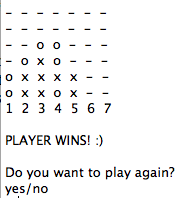
\includegraphics[scale=0.6]{jeu1} \\
	\textbf{Jeu d'esssai 1}
\end{center}
\begin{center}
	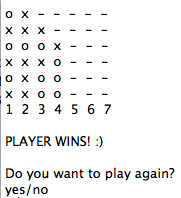
\includegraphics[scale=0.7]{jeu2} \\
	\textbf{Jeu d'esssai 2}
\end{center}
Comme on peut le voir dans les deux jeux d'essai, l'ordinateur a systématiquement tenté de bloquer l'avance du joueur adversaire en insérant un jeton au-dessus de celui du joueur (voir jeu 1 colonne 2 et 3, jeu 2 colonne 1). Aussi, on voit que l'ordinateur a bloquer un coup gagnant du joueur adverse. En effet, dans le jeu 1 à la colonne 3, l'ordinateur a bloquer le joueur humain l'empêchant de gagner la partie ne alignant 4 jetons dans la colonne 3. De plus, on voit dans le jeu 1 que l'ordinateur après avoir bloqué les coups de l'adverse, a tenter de gagner la partie en alignant 4 jetons dans la diagonale partant de la colonne 1 à la colonne 3. \\

Voici un autre jeu d'essai, ici gagné par l'ordianteur : \\
\begin{center}
	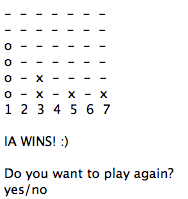
\includegraphics[scale=0.8]{jeu3} \\
	\textbf{Jeu d'esssai 3}
\end{center}
Dans cette partie, le joueur humain a placé les pions n'importe où pour voir le comportement de l'ordinateur. On peut donc voir que l'ordinateur a détecté que le joueur humain plaçait ses jetons sans vraiment de logique. Au lieu de bloquer ses coups, l'ordinateur a alors tenté de remporter la partie en alignant 4 jetons dans la même colonne, ici la colonne 1. \\

Dans les trois jeux d'essai observés, on voit que l'ordinateur a exactement le comportement voulu. Il bloque l'adversaire quand celui-ci fait un mouvement qui pourrait le faire gagner, l'ordinateur tente lui-même d'augmenter ses chances de gagner en alignant ses jetons et que l'ordinateur bloque les coups gagnants de l'adversaire. 

\section*{Conclusion}
Ce travail a permis d’explorer en profondeur un problème requérant l’utilisation de l’intelligence artificielle. Le problème consistant à un jeu comme Puissance 4 est certes simple, mais permet de faire une bonne introduction aux différentes techniques utilisées dans ce domaine et au langage de programmation Prolog.\\

En effet, programmer le jeu pour ce travail a demandé d’effectuer des recherches sur différents aspects du langage pour réaliser la programmation des différents composants. Les différents exemples du cours ont cependant permis d’avoir une base sur laquelle se fonder pour le reste du travail. La programmation fut la partie la plus difficile du travail à réaliser et le programme résultant n’est surement pas la manière la plus optimale de procéder. Il serait certainement intéressant de regarder ce code et peut-être même de regarder ce qui peut être amélioré lorsque notre connaissance de Prolog sera plus développée. \\

L’utilisation de la technique minimax pour la décision des mouvements de joueur ordinateur nous a permis d’explorer cette dernière à l’aide d’un exemple concret. Il y a certainement plusieurs autres manières de résoudre le problème, mais cette technique est simple, semble bien marché et elle s’applique très bien au jeu choisi dans ce travail. Il pourrait être intéressant de tester avec d’autre technique et d’autre fonction heuristique pour comparer les résultats.\\

Ce fut donc un travail en apparence simple, mais qui a demandé de développer en profondeur notre compréhension des différents éléments vus dans le cours. 

\newpage

\section{READ ME}
\textbf{Connect 4} \\

Travail pratique 1 du cours d'Intelligence artificielle IFT-2003 donné par Laurence Capus. 
Ce travail consistait à créer un jeu intelligent joueur versus oridnateur qui utilise des techniques 
d'intelligence artificielle. Le jeu choisi est Connect 4 ou Puissance 4. \\

\textbf{How to play} \\

Ouvrir SWI-Prolog. \\

Entrer le path du fichier tp2.pl ci-joint. Par exemple : \\

$['/Users/Catherine/connect4_tp/tp2.pl'].$ \\

Pour jouer au jeu, il suffit d'entrer la commande : \\

$play.$ \\

Il est maintenant l'heure de jouer :) \\

\textbf{Built With} \\

SWI-Prolog(http://www.swi-prolog.org/) \\

\textbf{Authors}
\begin{enumerate}
\item Catherine Asselin
\item Jérémie Lapointe
\item Patrick Voyer
\item Petru Lungu
\end{enumerate}

\end{document}
